% Intended LaTeX compiler: xelatex
\documentclass[12pt,notes]{beamer}
\usepackage{graphicx}
\usepackage{longtable}
\usepackage{wrapfig}
\usepackage{rotating}
\usepackage[normalem]{ulem}
\usepackage{amsmath}
\usepackage{amssymb}
\usepackage{capt-of}
\usepackage{hyperref}
\institute{}
\usepackage[danish]{babel}
\usepackage{mathtools}
\usetheme[progressbar=frametitle,block=fill,numbering=none]{metropolis}
\usepackage{hyperref}
\hypersetup{colorlinks, linkcolor=black, urlcolor=blue}
\titlegraphic{\begin{tikzpicture}[overlay,remember picture] \coordinate (logo) at ([xshift=-.07cm,yshift=-.07cm]current page.south west); \node [anchor=south west] at (logo) {
\includegraphics[width=2cm]{img/erasmus_plus.jpg}}; \end{tikzpicture}}
\logo{\begin{tikzpicture}[overlay,remember picture] \coordinate (logo) at ([xshift=.0cm,yshift=.0cm]current page.south west); \node [anchor=south west] at (logo) {
\includegraphics[width=2cm]{img/erasmus_plus.jpg}}; \end{tikzpicture}}
\usetheme{default}
\author{Erasmus+}
\date{28th and 29th of march}
\title{Breaks and brain breaks}
\subtitle{QuTe - Copenhagen}
\hypersetup{
 pdfauthor={Erasmus+},
 pdftitle={Breaks and brain breaks},
 pdfkeywords={},
 pdfsubject={},
 pdfcreator={Emacs 28.2 (Org mode 9.5.5)}, 
 pdflang={Danish}}
\begin{document}

\maketitle

\begin{frame}[label={sec:org77344f3}]{}
\section{09:00 - Let's begin!}
\begin{center}
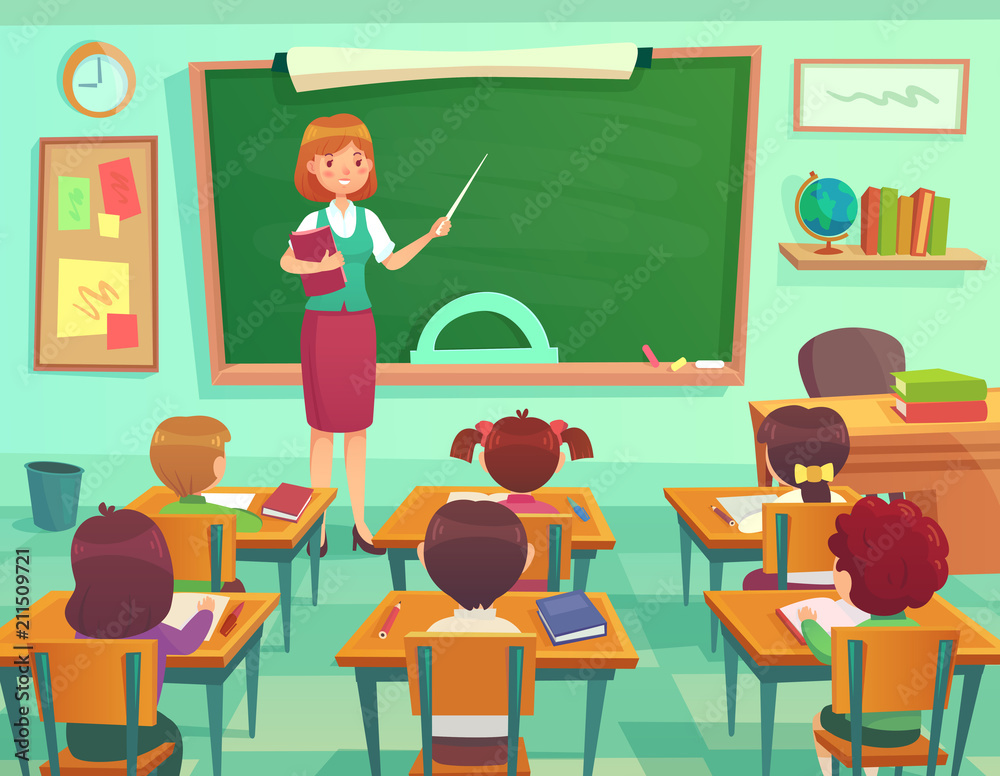
\includegraphics[width=7cm]{./img/lets_begin.jpg}
\end{center}
\end{frame}

\begin{frame}[label={sec:org659fa2d}]{}
\section{09:45 - Break time!}

\begin{center}
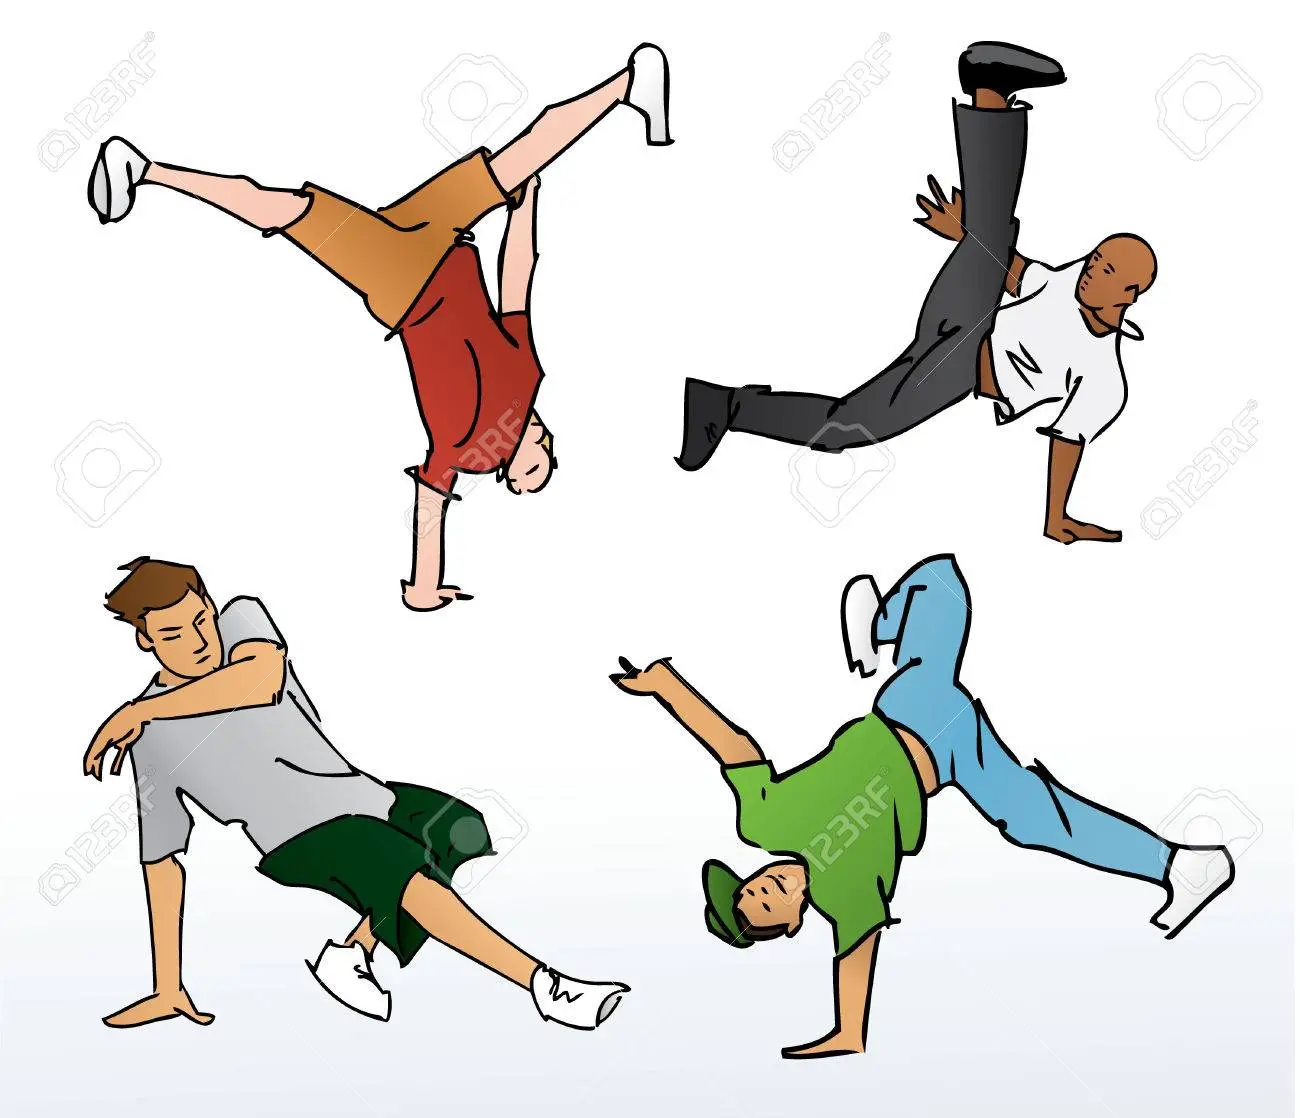
\includegraphics[width=5cm]{./img/break_dancing.png}
\end{center}
\end{frame}

\begin{frame}[label={sec:org881afa8}]{}
\section{10:00 - Break is over}

\begin{center}

\includegraphics[width=6cm]{./img/Full-Speed-Ahead.jpg}
\end{center}
\end{frame}


\begin{frame}[label={sec:org49efbc2}]{}
\section{Finger control!}

\begin{center}
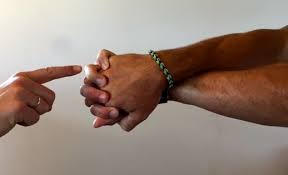
\includegraphics[width=8cm]{./img/finger_control.jpeg}
\end{center}

\note{Note for the exercise
\begin{itemize}
\item Fold fingers
\item First: One student \alert{points} and \alert{touches} the finger to move.
\item Next: One student \alert{points} but does not touch the finger to move.
\item Last: One student \alert{tells} which finger to move.
\end{itemize}}
\end{frame}

\begin{frame}[label={sec:org2d2b88d}]{}
\section{11:30 - Lunch break!}

\begin{center}
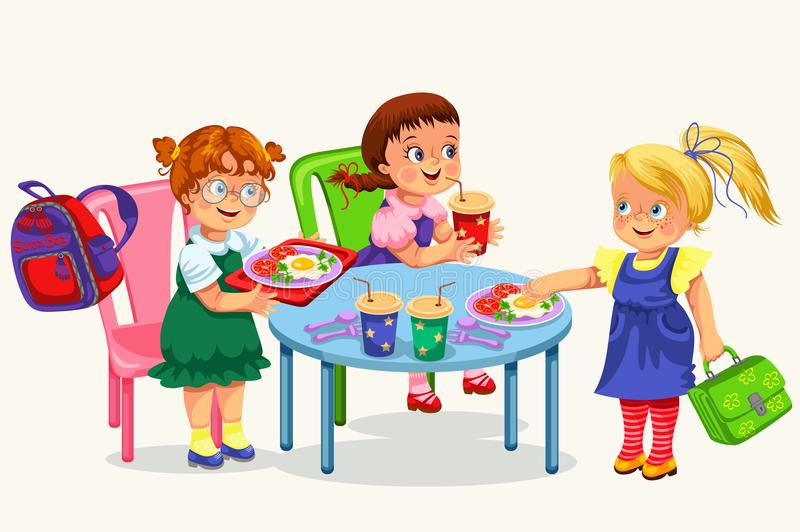
\includegraphics[width=7cm]{./img/lunch_break.jpg}
\end{center}
\end{frame}

\begin{frame}[label={sec:orga145850}]{}
\section{12:00 - On your mark, get set, GO!}

\begin{center}
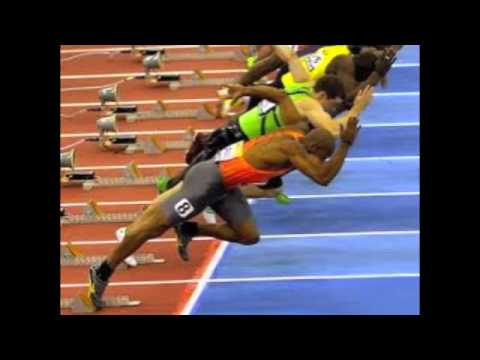
\includegraphics[width=7cm]{./img/on_your_mark_get_set_go.jpg}
\end{center}
\end{frame}

\begin{frame}[label={sec:org87750d9}]{}
\section{Shoot the rabbit!}

\begin{center}
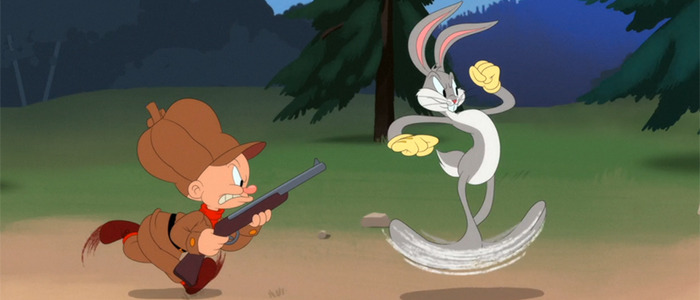
\includegraphics[width=8cm]{./img/shoot_the_rabbit.jpg}
\end{center}

\note{Note for the exercise
\begin{columns}
\begin{column}{0.5\columnwidth}
\begin{itemize}
\item Let the students practice the two signs with the hands.
\item Say it out loud: "Shoot, shoot, shoot the rabbit".
\item When saying \alert{rabbit} change the signs on the hands.
\item Speed up the exercise.
\end{itemize}
\end{column}
\begin{column}{0.5\columnwidth}
\begin{center}
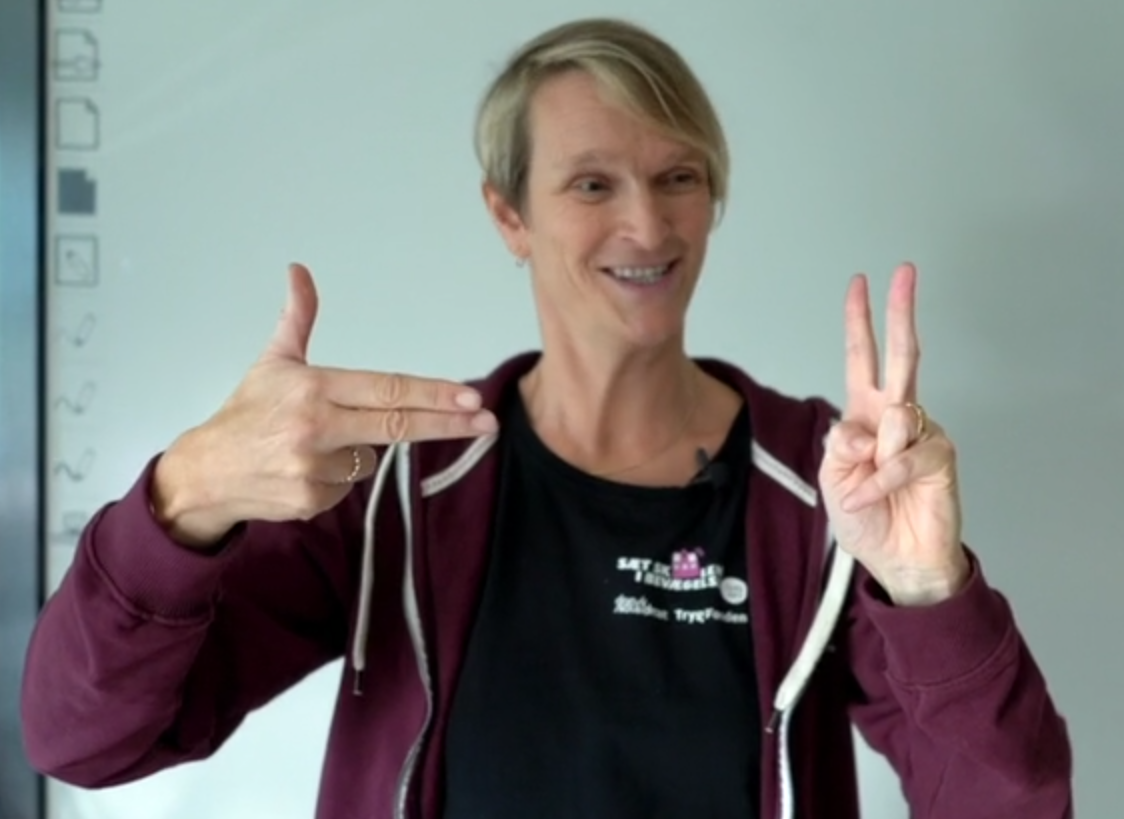
\includegraphics[width=\linewidth]{./img/shoot_the_rabbit_note.png}
\end{center}
\end{column}
\end{columns}}
\end{frame}

\begin{frame}[label={sec:org4fc9927}]{}
\section{13:30 - Break time!}

\begin{center}

\includegraphics[width=8cm]{./img/time_for_a_break.jpg}
\end{center}
\end{frame}

\begin{frame}[label={sec:org2e92016}]{}
\section{13:40 - Let's start again}
\begin{center}

\includegraphics[width=7cm]{./img/start_again.png}
\end{center}
\end{frame}

\begin{frame}[label={sec:org9769178}]{}
\section{14:25 - School's out - Next up bowling}

\begin{center}
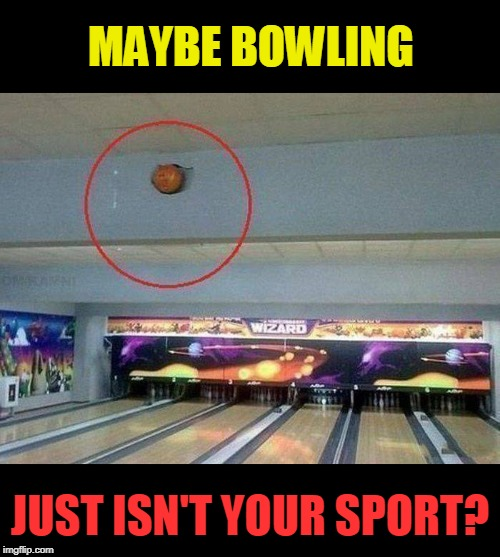
\includegraphics[width=5.5cm]{./img/bowling.jpeg}
\end{center}
\end{frame}

\begin{frame}[label={sec:orga603dea}]{}
\section{09:00 - Welcome back to the future!}

\begin{center}

\includegraphics[width=8cm]{./img/back_to_the_future.jpeg}
\end{center}
\end{frame}
\begin{frame}[label={sec:orge18bfb6}]{}
\section{09:45 - Break time!}

\begin{center}
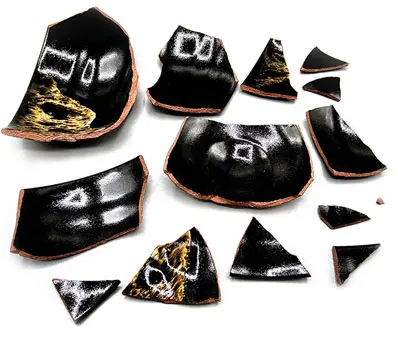
\includegraphics[width=6cm]{./img/kintsugi_broken.png}
\end{center}
\end{frame}

\begin{frame}[label={sec:orgb32133c}]{}
\section{10:00 - Break is over!}

\begin{center}
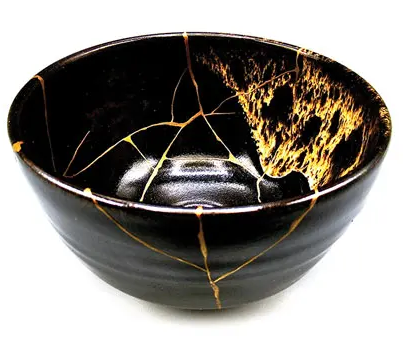
\includegraphics[width=6cm]{./img/kintsugi_repaired.png}
\end{center}
\end{frame}

\begin{frame}[label={sec:org49ce381}]{}
\section{The counting curse}

\begin{center}
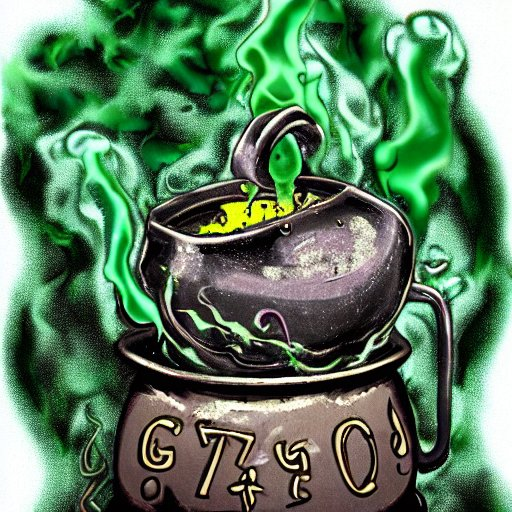
\includegraphics[width=5cm]{./img/counting_curse.jpeg}
\end{center}

\note{Note for the exercise
\footnotesize
\begin{itemize}
\item Split the class in two groups.
\item Each group gathers in a circle facing inwards.
\item Each group counts to 21 but only with one student may speak at a time.
\item If two students speak at the same time the group must start over.
\item If three or more students speak at the same time every student in the group must do 1-5 \alert{burpees}.
\item Make the groups do the exercise with eyes closed or similar challenges.
\end{itemize}}
\end{frame}
\begin{frame}[label={sec:orgc38d8df}]{}
\section{11:30 - Lunch break}

\begin{center}
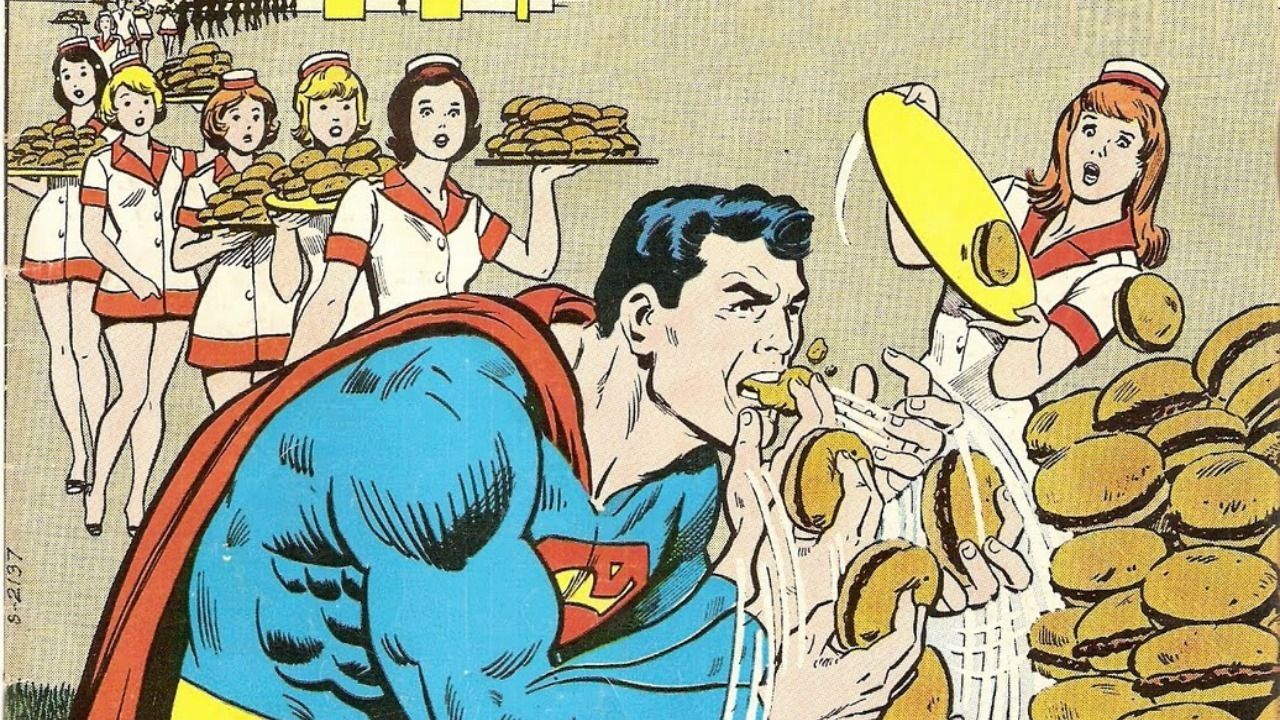
\includegraphics[width=8cm]{./img/superman_lunch.jpg}
\end{center}
\end{frame}

\begin{frame}[label={sec:org945b859}]{}
\section{12:00 - Let's start again.}

\begin{center}
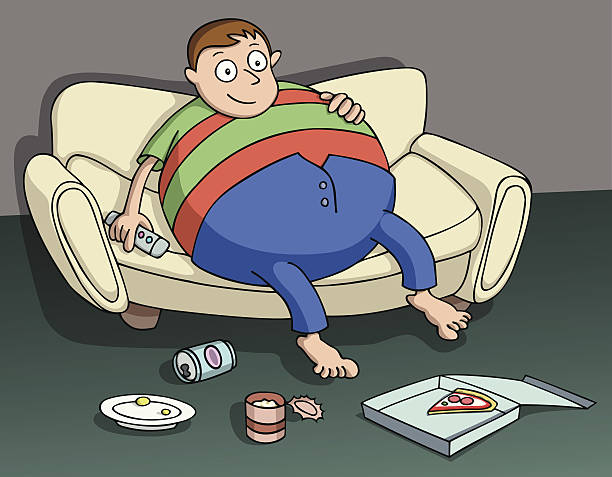
\includegraphics[width=7cm]{./img/after_lunch.jpg}
\end{center}
\end{frame}

\begin{frame}[label={sec:org88be933}]{}
\section{Hold the paper}

\begin{center}

\includegraphics[width=8cm]{./img/hold_the_paper.png}
\end{center}

\note{Note on the exercise
\begin{itemize}
\item The students should split up in groups of two.
\item Each group should hold a piece of a4 paper between their hands. One hand from each group member.
\item The exercise is now for the group to move the piece of paper down and in between each of the members legs withou letting go of the paper.
\item Variation: Form bigger groups which should in circles. Let the paper (or more papers) move between the legs around in the circle.
\end{itemize}}
\end{frame}

\begin{frame}[label={sec:org4e308c6}]{}
\section{13:30 - Break time!}
\begin{center}

\includegraphics[width=8cm]{./img/take_a_break.jpg}
\end{center}
\end{frame}

\begin{frame}[label={sec:org17b0607}]{}
\section{13:40 - Let's start again.}
\begin{center}

\includegraphics[width=7cm]{./img/lets_start_again.jpg}
\end{center}
\end{frame}

\begin{frame}[label={sec:org1bdfb01}]{}
\section{14:25 - School's out - See you tomorrow}

\begin{center}

\includegraphics[width=8cm]{./img/schools_out.jpg}
\end{center}
\end{frame}
\end{document}